% !TeX spellcheck = en_US
% !TeX root = ../main.tex
\section{Methods}
\label{sec:methods}

Since the legal system produces a diverse set of outputs, many of which are rich in internal structure, a methodological framework for its dynamic network analysis must allow for many different foci and units of analysis. 
Our methods are designed to match this need, enabling us to describe the legal system and its evolution in its entirety (\emph{macro level}), through selected sets of legal documents (\emph{meso level}), or using individual documents and their substructures \emph{(micro level}), 
all while integrating documents of potentially different types.
More precisely, we provide tools for measuring 
\begin{enumerate}
	\item the \emph{growth} of the legal system (\ref{subsec:methods:growth}),
	\item the macro-level, meso-level, and micro-level \emph{connectivity} of the legal system (\ref{subsec:methods:connectivity}), and 
	\item the \emph{evolution} of individual units of law (e.g., single statutes, single regulations, or their sections or chapters) in the legal system (\ref{subsec:methods:profiles}).
\end{enumerate}
While most network analytical tools we employ are conceptually simple, the challenge lies in selecting adequate units of analysis and metrics allowing for substantive interpretation.
In the following, we refer to the object of study as \emph{the legal system} for brevity, 
but one should keep in mind that this system is explored through the window provided by the document collection underlying the analysis (cf.~Figure~\ref{fig:legal-system}), 
and therefore can also refer to a \emph{national legal system}.

\vspace*{6pt}
\subsection{Growth}
\label{subsec:methods:growth}

As detailed in Section~\ref{subsec:data:model}, despite their diversity, the typical outputs of the legal system have \emph{hierarchy}, \emph{sequence}, and \emph{reference} as common structural features, and they also all contain \emph{text}. 
Therefore, to assess the growth of the legal system, we track the number of tokens (roughly corresponding to words), the number of structural elements (i.e., hierarchical structures), and the number of references between documents of the same type at the documents' sequence level (e.g., the section level for statutes and regulations) across all documents in the collection, separately for each document type and across all temporal snapshots (e.g., all years). 
For the token counts, we concatenate the text of all materials for one snapshot and document type and split on whitespace characters. 
For a given document type, the structural element counts reflect the number of nodes of that type, and the reference counts reflect the number of reference edges between nodes of that type in our graphs.
These measures give a first, high-level idea of how the legal system evolves, and the aggregation by document type allows us to uncover, e.g., differences in growth rates. 

\begin{figure} 
	\centering
	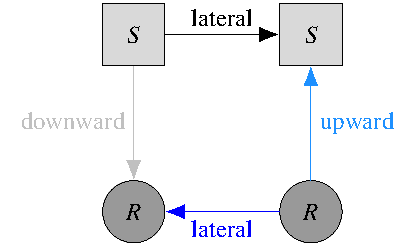
\includegraphics[width=0.5\textwidth]{figure_3}
	\caption{Differentiation of reference types for a document collection containing two types of documents: statutes and regulations. 
	Light grey squares marked $S$ represent sections of statutes, dark grey circles marked $R$ represent sections of regulations. 
	Given that statutes stand above regulations in the hierarchy of legal rules, 
	a reference from a statute to a regulation is \emph{downward} (silver), a reference from a regulation to a statute is \emph{upward} (light blue), 
	and references between documents of the same type are \emph{lateral} (black and blue).}\label{fig:crossref-differentiation}
\end{figure}

To explore the relevance of references between documents of different types, if the document collection contains $x$ types of documents, we distinguish between $x^2$ types of references. 
Figure~\ref{fig:crossref-differentiation} illustrates the idea for $x = 2$ with statutes and regulations as document types.
We count the number of references of each type for each temporal snapshot.

Raw reference counts do not show how the incoming and outgoing references are distributed across the individual sequence-level items. 
The user experience of a legal system, however, depends crucially on these distributions: 
If the typical item on the sequence level has very few outgoing references, the \emph{expected} cost of navigating the law is much smaller than if the outgoing references are uniformly distributed, 
and if the distribution of incoming references is very skewed, when reading the law, we are much more likely to encounter a few prominent sequence-level items than a large number of less prominent ones
(of course, the \emph{actual} cost of the user also depends on the size of the items to be navigated, which can vary widely, e.g., amongst the sections in the USC).
Therefore, we inspect the evolution of the in-degree distribution and the out-degree distribution of the subgraph induced by the reference edges.
We compute these distributions separately for each combination of reference edge types (e.g., considering any combination of the reference types depicted in Figure~\ref{fig:crossref-differentiation} for a document collection containing statutes and regulations) and across all snapshots.
This allows us to evaluate whether growth in the number of references further amplifies differences in the prominence of different parts of the law, 
which would be reflected in a lengthening or thickening of the distributions' tails, and to assess how this affects the navigability of a legal system.

\vspace*{6pt}
\subsection{Connectivity}
\label{subsec:methods:connectivity}

When exploring the connectivity of the legal system over time, we distinguish between macro-level connectivity (\ref{subsubsec:methods:connectivity:macro}), meso-level connectivity (\ref{subsubsec:methods:connectivity:meso}), and micro-level connectivity (\ref{subsubsec:methods:connectivity:micro}). 

\vspace*{6pt}
\subsubsection{Macro-level connectivity}
\label{subsubsec:methods:connectivity:macro}

Investigating connectivity at the macro level helps us understand how information in the legal system is organized and processed. 
As the basis of all analyses, we consider the graph induced by the structural items on the documents' sequence level (referred to as \emph{seqitems} in \cite{katz2020}) as nodes and the references between them as edges. 
For each snapshot, we count the number of non-trivial connected components (i.e., components with more than one node). 
Furthermore, we compute the fraction of nodes in the largest (weakly) connected component, 
the fraction of nodes in satellites, i.e., non-trivial components that are not the largest connected component, 
and the fraction of isolated nodes. 
We do this for the graph containing nodes of all document types as well as for the graphs containing only nodes of a single document type. 
These statistics provide a high-level overview of the system's information infrastructure and how it changes over time, 
and they enable a differentiated assessment of the role of documents of different types. 

For a more detailed picture, we draw on concepts introduced in the study of the Web graph \cite{broder2000}, which have also proven useful in the analysis of complex and self-organizing systems, e.g., in biology \cite{friedlander2015,csete2004,ma2003}. 
More precisely, we analyze the largest connected component of each of the sequence-level reference graphs, 
tracking the fraction of nodes contained in its strongly connected component, its in-only component (i.e., the nodes which can reach \emph{to} but cannot be reached \emph{from} the strongly connected component), its out-only component (i.e., the nodes which can be reached \emph{from} but cannot reach \emph{to} the strongly connected component), and its tendrils and tubes (whatever remains), 
again across all snapshots.
We ask to what extent the legal system has a bowtie structure (i.e., a small strongly connected core joined by larger in-only and out-only components), which has been associated with ``effective trade-offs among efficiency, robustness and evolvability'' \cite{csete2004}, inter alia, in complex biological systems, and whether any empirical deviations from that structure are characteristic of legal information processing.

\vspace*{12pt}
\subsubsection{Meso-level connectivity}
\label{subsubsec:methods:connectivity:meso}

One fundamental question concerning a legal system's connectivity at the meso level is how it self-organizes into areas of law.
Existing taxonomies categorizing the law into distinct fields are largely based on tradition (e.g., the titles of the USC) or intuition (e.g., the thematic categories used by some legal database providers). 
Exploiting the connectivity provided by references between legal documents at the meso level, network analytical methods provide an alternative, data-driven approach to mapping the law.
To implement such an approach, 
we follow a multi-step procedure:
\begin{enumerate}
	\item We preprocess the graphs for each snapshot by taking the quotient graph at the granularity we are interested in (e.g., at the level of individual chapters for an analysis of the USC and the CFR).
	That is, we remove all nodes above and below that level and reroute all references outgoing from or incoming to a lower-level node to the node's unique ancestor that lies on the level of interest.\label{step:quotient} 
	\item We cluster each of the \emph{undirected} versions of the graphs from Step~\ref{step:quotient} separately using the \emph{Infomap} algorithm \cite{rosvall2008,rosvall2009} with a parametrization that mirrors domain knowledge, and passes sensitivity and robustness checks. 
	Leveraging the randomness inherent in this algorithm, we increase the robustness of the clustering for each graph by computing the \emph{consensus clustering} \cite{lancichinetti2012} of $1000$ \emph{Infomap} runs with different seeds, where two nodes are put into the same cluster if they are in the same cluster in $95~\%$ of all runs.
	We choose the \emph{Infomap} algorithm as our clustering algorithm because it is scalable, has a solid information-theoretic foundation, and mirrors the process in which users like lawyers navigate law (inter alia, by identifying a relevant section of a statute, reading that section, then potentially following a reference).\label{step:clustering} 
	\item We compute pairwise alignments between the clusterings of all temporally adjacent snapshots based on the nodes of the \emph{unpreprocessed} graphs that wrap text (for details on our alignment procedure, see Section~4.3.1 in the \thesi).
	This is most relevant for collections containing documents that can change over time (e.g., statutes and regulations), and it allows us to assess, inter alia, what amount of text from a cluster $A$ in year $y$ is contained in a cluster $B$ in year $y+1$.\label{step:alignment}   
	\item We use the clusterings from Step~\ref{step:clustering} and the alignments from Step~\ref{step:alignment} to define a \emph{cluster family graph} as introduced in \cite{katz2020}. 
	This graph contains all clusters from all snapshots as nodes, and two clusters $A$ and $B$ are connected by a (weighted) edge if $A$ lies in snapshot $y$, $B$ lies in snapshot $y+1$, at least $p~\%$ of the tokens from $A$ are contained in $B$, and at least $p~\%$ of the tokens from $B$ are contained in $A$, where $p$ is chosen based on the analytical resolution we are interested in.\label{step:familygraph}
	\item We define a \emph{cluster family} as a connected component in a cluster family graph from Step~\ref{step:familygraph} and compute, for each cluster family in each year, the number of tokens it contains from each document type.\label{step:family}
\end{enumerate}
This process is a variant of the family graph construction developed for statutes in \cite{katz2020}, 
with the modification that we now allow for input data containing documents of different types.
It results in a dynamic, data-driven map of the legal system that accounts for the information provided by the references between its documents.

\vspace*{6pt}
\subsubsection{Micro-level connectivity}
\label{subsubsec:methods:connectivity:micro}

At the micro level, the connectivity created by references allows us to assess the roles of individual units of law. 
Regardless of the level at which we aggregate the references between documents, 
the shapes of the nodes' neighborhoods at that level contain valuable information about their function in the legal system. 
This information is partly accounted for in the meso-level connectivity assessment, which leverages local \emph{density}.
While local density can help us find out which nodes interact strongly, local \emph{sparsity} lets us identify nodes that play a particularly prominent role for the information flow in the network: 
If a node's neighbors are themselves only very sparsely connected (i.e., their neighbors almost form an independent set), the node provides an important \emph{bridge} between them.
We call the ego graph of such a node a \emph{star}, 
with the node as its \emph{hub} and the node's neighbors as the \emph{spokes}.

In directed graphs, we can classify stars according to the ratio between the hub's in-degree and the hub's out-degree as depicted in Figure~\ref{fig:star-types}.
More precisely, we define the type of a star $s$ with hub $v$ as follows:
\begin{align*}
	\text{type}(s) := \begin{cases}
		\frac{\delta^-(v)}{\delta^+(v)} \geq 10&\text{sink}\\
		\frac{1}{10} < \frac{\delta^-(v)}{\delta^+(v)} < 10&\text{hinge}\\
		\frac{\delta^+(v)}{\delta^-(v)} \geq 10&\text{source},
	\end{cases}
\end{align*}
where $\delta^+(v)$ is $v$'s out-degree and $\delta^-(v)$ is $v$'s in-degree.
In the legal system, the type of a star captures the hub's role in mediating the information flow in its neighborhood.

\begin{figure}
	\centering
	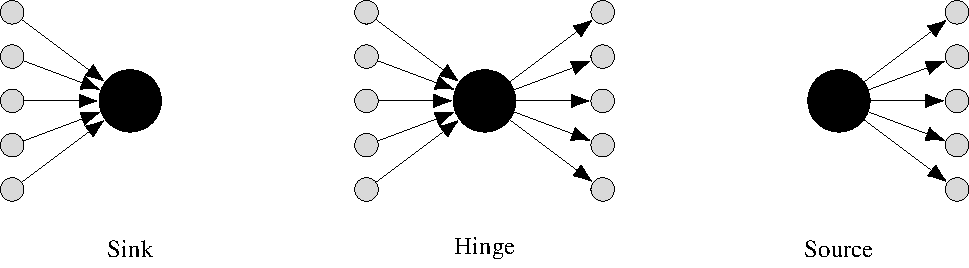
\includegraphics{figure_4}
	\caption{Star types. 
	If the hub's in-degree is at least ten times its out-degree, the star is a \emph{sink}. 
	If the hub's out-degree is at least ten times its in-degree, the star is a \emph{source}. 
	Otherwise, the star is a \emph{hinge}.}\label{fig:star-types}
\end{figure}

To identify and classify stars in the legal system at the documents' sequence level,
for each snapshot, we create the ego graph for each node $v$ in the graph induced by the reference edges (where we exclude parallel edges). 
We then iteratively remove the node $w$ that is connected to most of $v$'s neighbors while $w$ is connected to more than $5~\%$ of $v$'s neighborhood (excluding $w$), and keep the ego graph if it has a certain minimum size determined by the size of the collection (e.g., $10$ nodes for collections with several thousands of items on the sequence level).
The stars produced in this way contain no spoke that is connected to more than $5~\%$ of the other spokes, and we classify them to identify those sequence-level items that are vital to the information flow in their neighborhoods and to describe the type of mediation they perform.
To find stars at levels above the documents' sequence level, we can apply the methodology just described on graphs that aggregate references at those levels (e.g., on the quotient graphs described in Section~\ref{subsubsec:methods:connectivity:meso}).

\vspace*{12pt}
\subsection{Profiles}
\label{subsec:methods:profiles}

To assess the evolution of individual units of law (e.g., individual court decisions or chapters of a regulation) in the legal system, we create profiles of these units covering all temporal snapshots in the document collection under study.
More specifically, based on the quotient graphs that are created on the level of our unit of interest and contain only reference edges (like the preprocessed graphs described in Step~\ref{step:quotient}, Section~\ref{subsubsec:methods:connectivity:meso}), 
we track ten statistics in five groups (note that not all of these statistics can change over time for units of all legal document types):
\begin{enumerate}
	\item the number of tokens and the number of unique tokens,
	\item the number of items above, on, and below the sequence level (provided our unit of analysis lies above the sequence level),
	\item the number of self-loops,
	\item the weighted in- and out-degree (accounting for parallel edges), and
	\item the binary in- and out-degree (excluding parallel edges).
\end{enumerate} 

These statistics capture how the unit of law in focus evolves in size (number of tokens), 
topical breadth (number of unique tokens), 
structure (number of items above, on, and below the sequence level), 
self-referentiality (number of self-loops), 
scope of interdependence within the legal system (weighted in-degree and weighted out-degree), 
and diversity of interdependence within the legal system (binary in-degree and binary out-degree).
Finally, by constructing the ego graphs of the profiled unit for its out-neighborhood and its in-neighborhood and following the evolution of these ego graphs across snapshots,
we assess to what extent a profiled unit references which other units (\emph{reliance}) 
and to what extent it is referenced by which other units (\emph{responsibility}).
